\documentclass[tikz,border=12pt]{standalone}
\usepackage{tikz}
\usepackage{fontawesome5}
\usepackage{amsmath,amssymb}
\usetikzlibrary{arrows.meta,positioning,fit,backgrounds,calc,shadows,shapes.geometric}

% Color definitions
\definecolor{lavenderDark}{RGB}{15, 44, 89}
\definecolor{lavenderDeep}{RGB}{10, 28, 58}
\definecolor{lavenderMedium}{RGB}{29, 78, 158}
\definecolor{lavenderLight}{RGB}{240, 246, 255}
\definecolor{lavenderBorder}{RGB}{180, 205, 237}
\definecolor{lavenderAccent}{RGB}{2, 132, 199}
\definecolor{prismNavy}{RGB}{15, 44, 89}
\definecolor{prismBlue}{RGB}{29, 78, 158}
\definecolor{prismTeal}{RGB}{13, 148, 136}
\definecolor{prismMint}{RGB}{236, 253, 245}
\definecolor{prismGold}{RGB}{217, 119, 6}
\definecolor{prismDark}{RGB}{15, 23, 42}
\definecolor{prismLight}{RGB}{248, 250, 252}
\definecolor{statusFail}{RGB}{220, 38, 38}
\definecolor{cInput}{RGB}{241, 245, 249}
\definecolor{cStem}{RGB}{224, 242, 254}
\definecolor{cStage1}{RGB}{209, 250, 229}
\definecolor{cStage2}{RGB}{254, 243, 199}
\definecolor{cHead}{RGB}{219, 234, 254}
\definecolor{cDeliverable}{RGB}{204, 251, 241}

\begin{document}
% Layered System Workflow for Voter Registration & Whitelisting
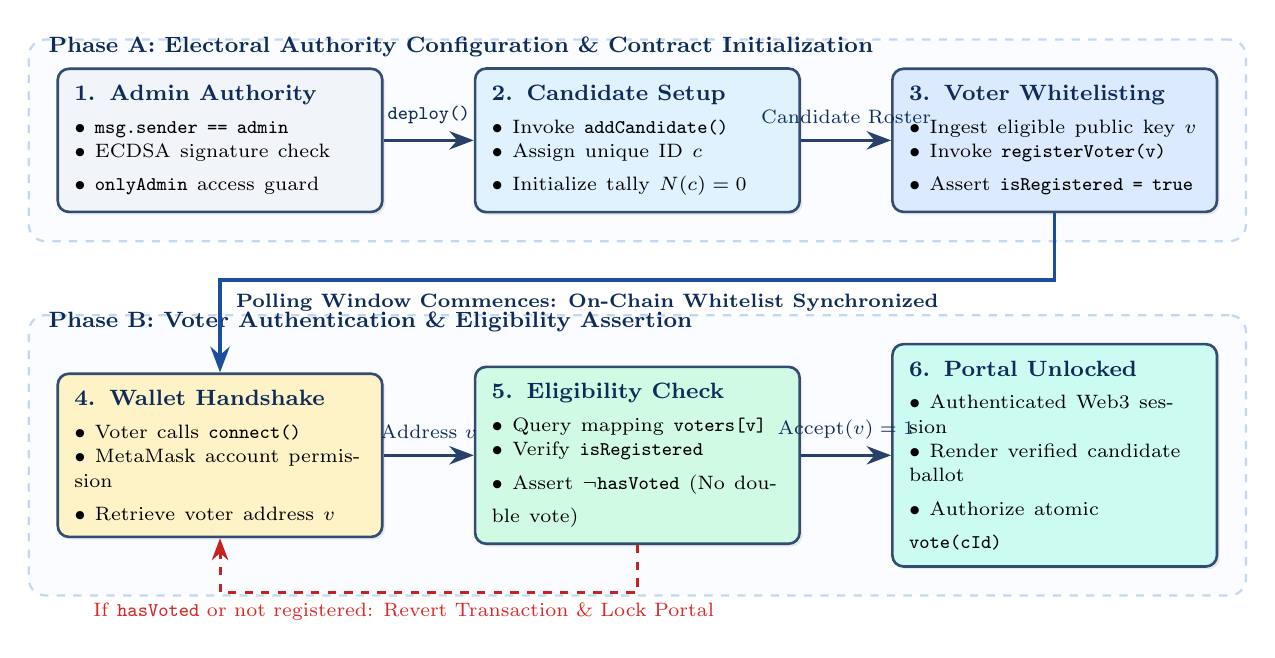
\begin{tikzpicture}[
    x=1cm, y=1cm,
    stepbox/.style={
        rectangle, draw=lavenderDark!85, line width=0.95pt, fill=white,
        rounded corners=4pt, inner sep=6pt, align=left,
        drop shadow={shadow xshift=1pt, shadow yshift=-1pt, opacity=0.15}
    },
    phasebox/.style={
        rectangle, draw=lavenderBorder!80, line width=0.8pt, fill=lavenderLight!35,
        rounded corners=6pt, inner sep=10pt, dashed
    },
    flowarr/.style={
        -{Stealth[scale=1.05]}, line width=1.2pt, draw=lavenderDark!90
    },
    dashloop/.style={
        -{Stealth[scale=1.0]}, line width=1.1pt, dashed, draw=prismBlue!90!black
    },
    revertarr/.style={
        -{Stealth[scale=1.0]}, line width=1.1pt, dashed, draw=statusFail!90!black
    }
]

    % =========================================================================
    % ROW 1: ADMINISTRATOR ELECTION SETUP PHASE
    % =========================================================================
    
    % Step 1: Admin Authority Verification
    \node [stepbox, fill=cInput, text width=3.7cm] (b1) at (-5.3, 2.0) {
        {\fontsize{8.5}{10.5}\selectfont\bfseries\color{lavenderDark}1. Admin Authority}\\[0.3em]
        \fontsize{7.2}{8.8}\selectfont
        $\bullet$ \texttt{msg.sender == admin}\\
        $\bullet$ ECDSA signature check\\
        $\bullet$ \texttt{onlyAdmin} access guard
    };

    % Step 2: Candidate Management
    \node [stepbox, fill=cStem, text width=3.7cm] (b2) at (0.0, 2.0) {
        {\fontsize{8.5}{10.5}\selectfont\bfseries\color{lavenderDark}2. Candidate Setup}\\[0.3em]
        \fontsize{7.2}{8.8}\selectfont
        $\bullet$ Invoke \texttt{addCandidate()}\\
        $\bullet$ Assign unique ID $c$\\
        $\bullet$ Initialize tally $N(c)=0$
    };

    % Step 3: Voter Whitelisting
    \node [stepbox, fill=cHead, text width=3.7cm] (b3) at (5.3, 2.0) {
        {\fontsize{8.5}{10.5}\selectfont\bfseries\color{lavenderDark}3. Voter Whitelisting}\\[0.3em]
        \fontsize{7.2}{8.8}\selectfont
        $\bullet$ Ingest eligible public key $v$\\
        $\bullet$ Invoke \texttt{registerVoter(v)}\\
        $\bullet$ Assert \texttt{isRegistered = true}
    };

    % Phase 1 Background Box
    \begin{scope}[on background layer]
        \node [phasebox, fit=(b1)(b2)(b3), label={[font=\fontsize{7.8}{9.5}\selectfont\bfseries\color{lavenderDark}, anchor=west, xshift=4pt, yshift=-3pt]north west:Phase A: Electoral Authority Configuration \& Contract Initialization}] (p1) {};
    \end{scope}

    % Row 1 Connectors
    \draw [flowarr] (b1) -- node[above=2pt, font=\fontsize{6.8}{8.0}\selectfont, text=prismNavy] {\texttt{deploy()}} (b2);
    \draw [flowarr] (b2) -- node[above=2pt, font=\fontsize{6.8}{8.0}\selectfont, text=prismNavy] {Candidate Roster} (b3);

    % =========================================================================
    % ROW 2: VOTER AUTHENTICATION & ELIGIBILITY VERIFICATION PHASE
    % =========================================================================

    % Step 4: MetaMask Handshake
    \node [stepbox, fill=cStage2, text width=3.7cm] (b4) at (-5.3, -2.0) {
        {\fontsize{8.5}{10.5}\selectfont\bfseries\color{lavenderDark}4. Wallet Handshake}\\[0.3em]
        \fontsize{7.2}{8.8}\selectfont
        $\bullet$ Voter calls \texttt{connect()}\\
        $\bullet$ MetaMask account permission\\
        $\bullet$ Retrieve voter address $v$
    };

    % Step 5: Eligibility Verification
    \node [stepbox, fill=cStage1, text width=3.7cm] (b5) at (0.0, -2.0) {
        {\fontsize{8.5}{10.5}\selectfont\bfseries\color{lavenderDark}5. Eligibility Check}\\[0.3em]
        \fontsize{7.2}{8.8}\selectfont
        $\bullet$ Query mapping \texttt{voters[v]}\\
        $\bullet$ Verify \texttt{isRegistered}\\
        $\bullet$ Assert $\neg\texttt{hasVoted}$ (No double vote)
    };

    % Step 6: Portal Access Unlocked
    \node [stepbox, fill=cDeliverable, text width=3.7cm] (b6) at (5.3, -2.0) {
        {\fontsize{8.5}{10.5}\selectfont\bfseries\color{lavenderDark}6. Portal Unlocked}\\[0.3em]
        \fontsize{7.2}{8.8}\selectfont
        $\bullet$ Authenticated Web3 session\\
        $\bullet$ Render verified candidate ballot\\
        $\bullet$ Authorize atomic \texttt{vote(cId)}
    };

    % Phase 2 Background Box
    \begin{scope}[on background layer]
        \node [phasebox, fit=(b4)(b5)(b6), label={[font=\fontsize{7.8}{9.5}\selectfont\bfseries\color{lavenderDark}, anchor=west, xshift=4pt, yshift=-3pt]north west:Phase B: Voter Authentication \& Eligibility Assertion}] (p2) {};
    \end{scope}

    % Row 2 Connectors
    \draw [flowarr] (b4) -- node[above=2pt, font=\fontsize{6.8}{8.0}\selectfont, text=prismNavy] {Address $v$} (b5);
    \draw [flowarr] (b5) -- node[above=2pt, font=\fontsize{6.8}{8.0}\selectfont, text=prismNavy] {$\text{Accept}(v)=1$} (b6);

    % =========================================================================
    % INTER-PHASE CONNECTORS & FEEDBACK
    % =========================================================================

    % Transition from Phase A to Phase B
    \draw [flowarr, line width=1.3pt, draw=prismBlue] (b3.south) -- ++(0,-0.85) -| (b4.north)
        node[pos=0.28, below=1pt, font=\fontsize{7.2}{8.8}\selectfont\bfseries, text=prismNavy] {Polling Window Commences: On-Chain Whitelist Synchronized};

    % Revert / Double-Voting Defense Branch
    \draw [revertarr] (b5.south) -- ++(0,-0.6) -| node[pos=0.28, below, font=\fontsize{6.8}{8.0}\selectfont, text=statusFail] {If \texttt{hasVoted} or not registered: Revert Transaction \& Lock Portal} (b4.south);

\end{tikzpicture}
\end{document}
